\begin{figure}[t]
  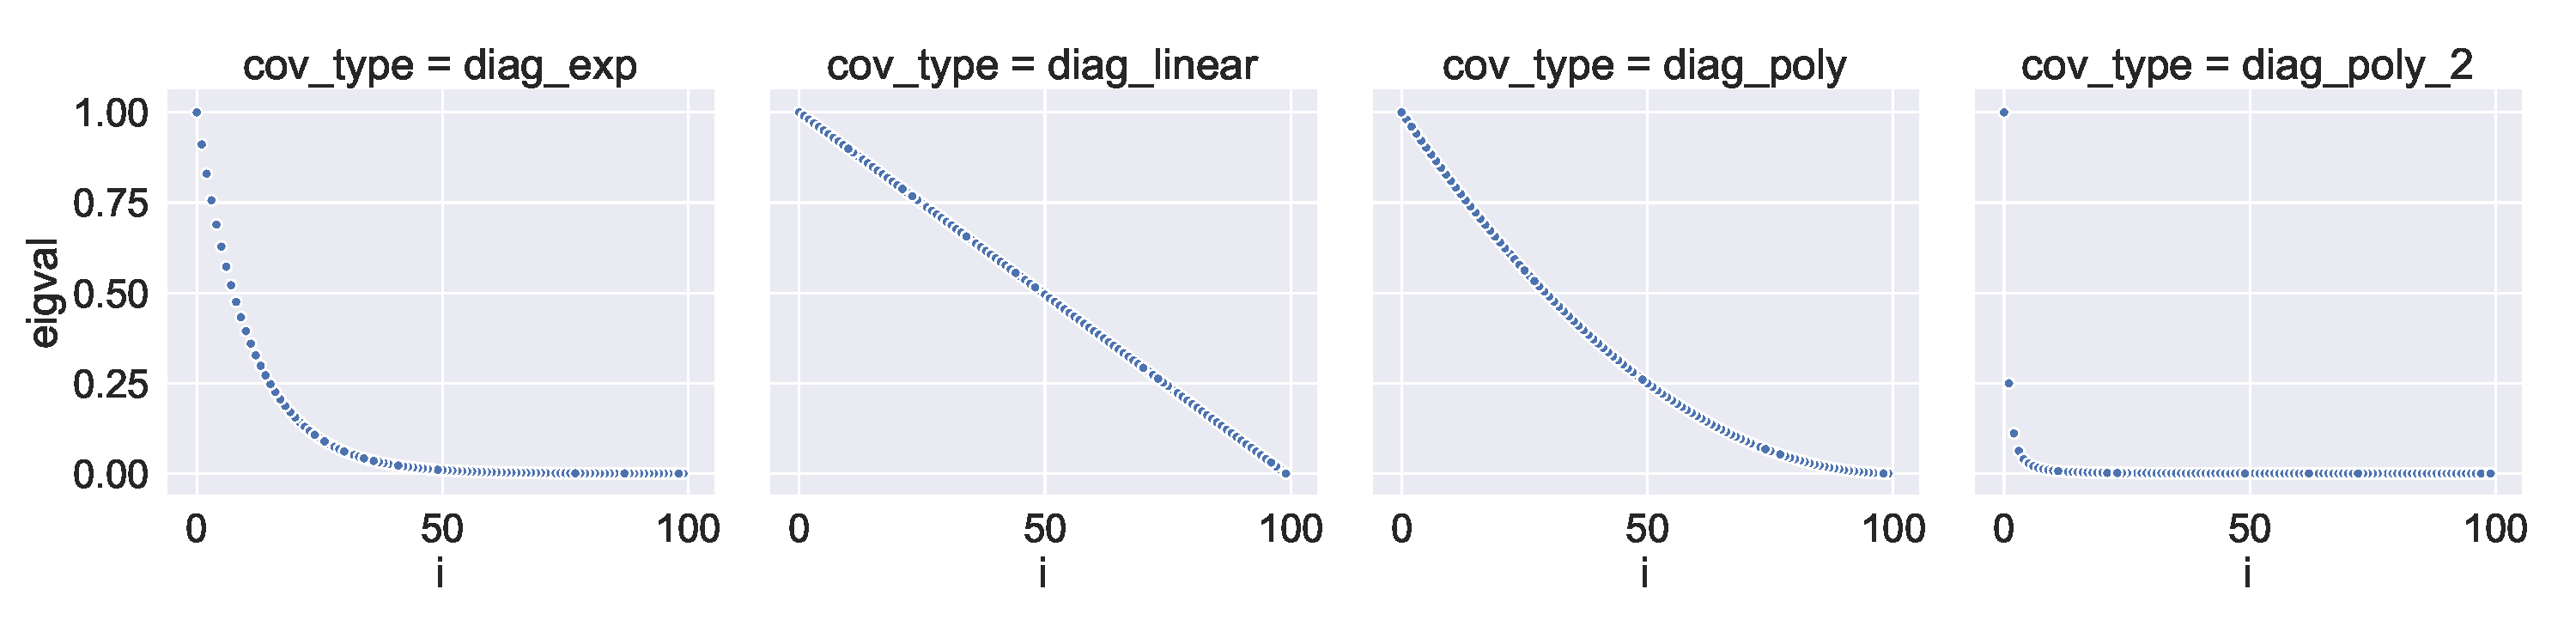
\includegraphics[width=\textwidth]{continuous_figures/decays.pdf}
  \vspace{-1cm}
  \caption{Scree-plots of $\Sigmab$ for the eigenvalue decays examined
    in our empirical valuations.
    % Here $d=100$ for visualization, whereas
    % our experiments increase $d$ while preserving the ratio $n/d$ and
    % the decay profile,
    % with $\lambda_{\text{max}}(\Sigmab) = 1$ to
    % $\lambda_{\text{min}}(\Sigmab) = 10^{-4}$.
  }
  \label{fig:eig-decays}
\end{figure}


\section{Empirical evaluation of asymptotic consistency}
\label{sec:asymp-conj-details}

% While Theorem~\ref{t:asymptotic} is a result on asymptotic consistency of the
% MSE, the proof (Appendix~\ref{sec:proof-of-t-asymptotic}) follows the standard
% decomposition of MSE in Equation~\ref{eq:mse-derivation} in the process
% establish consistency on the bias and variance terms independently.

% Recall that $\lambda_n=\frac {d-n}{\tr((\Sigmab+\lambda_n\I)^{-1})}$,
% so our surrogate MSE is recovered as
% $\sigma^2\Vc(\Sigmab,n)+\w^{*\top}\Bc(\Sigmab,n)\w^*$.
% % The expressions $\Vc(\Sigmab,n)$ and $\Bc(\Sigmab,n)$ and recover
% % surrogate MSE from Theorem \ref{t:mse} since $\lambda_n=\frac{\tr((\Sigmab+\lambda_n)^{-1})}{d-n}$.
% Lemmas \ref{c:wishart} and \ref{c:projection} provide new insights into classical matrix-variate
% distributions with extensive literature dedicated to them \citep[see,
% e.g.,][]{chikuse1990matrix,cook2011}.
%
%
%

%\section{Empirical evaluation of asymptotic consistency}

% Theorem \ref{t:asymptotic} shows that the surrogate MSE expressions
% derived in Theorem \ref{t:mse} are asymptotically consistent with the
% true MSE for the i.i.d.~design under a class of sub-gaussian data
% distributions.
In this section, we empirically quantify the convergence rates for
the asymptotic result of Theorem~\ref{t:asymptotic}.
% when $\mu$ is a centered multivariate% Gaussian $\Nc(\zero,\Sigmab).$
We focus on the under-determined regime (i.e.,
$n<d$) and separate the evaluation into the bias and
variance terms, following the MSE decomposition given
in \eqref{eq:mse-derivation}. Consider  $\X = \Z\Sigmab^{1/2} $, where the entries of $\Z$ are
i.i.d. standard Gaussian, and define:\vspace{-1mm}
\begin{enumerate}
  \item Variance discrepancy:\quad
    $\big|\frac{\E[\tr((\X^\top\X)^\dagger)]}{\Vc(\Sigmab,n)}-1\big|$ where
    $\Vc(\Sigmab,n)=\frac{1-\alpha_n}{\lambda_n}$.
  \item Bias discrepancy:\quad
     $\sup_{\w\in\R^d\backslash\{\zero\}}\big|\frac{\w^\top\E[\I-\X^\dagger\X]\w}
     {\w^\top\Bc(\Sigmab,n)\w} - 1\big|$
    where $\Bc(\Sigmab,n) = \lambda_n(\Sigmab+\lambda_n\I)^{-1}$.
  \end{enumerate}\vspace{-1mm}
   Recall that $\lambda_n=\frac {d-n}{\tr((\Sigmab+\lambda_n\I)^{-1})}$,
so our surrogate MSE can be written as
$\Mc=\sigma^2\Vc(\Sigmab,n)+\w^{*\top}\Bc(\Sigmab,n)\w^*$, and when both
discrepancies are bounded by $\epsilon$, then $(1-2\epsilon)\Mc\leq\MSE{\X^\dagger\y}\leq (1+2\epsilon)\Mc$.
In our experiments, we consider four standard eigenvalue decay profiles
for $\Sigmab$, including polynomial and exponential decay (see
 \Cref{fig:eig-decays} and \Cref{sec:eig-decay-details}).
\begin{figure} %[ht]
  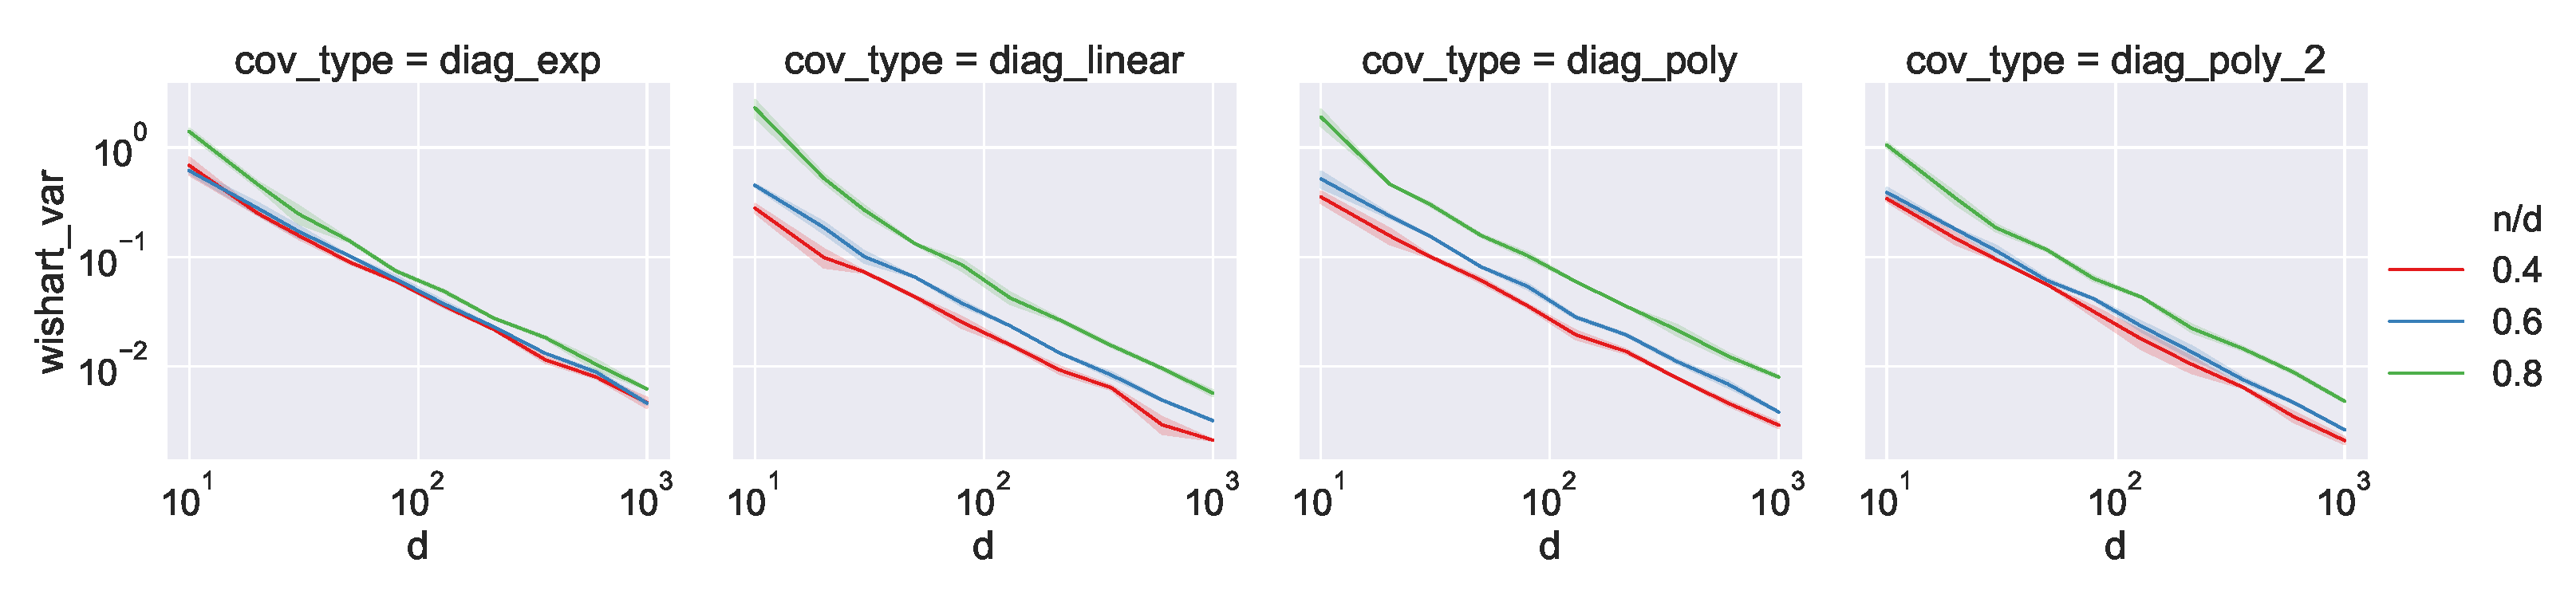
\includegraphics[width=\textwidth]{continuous_figures/wishart_var.pdf}
  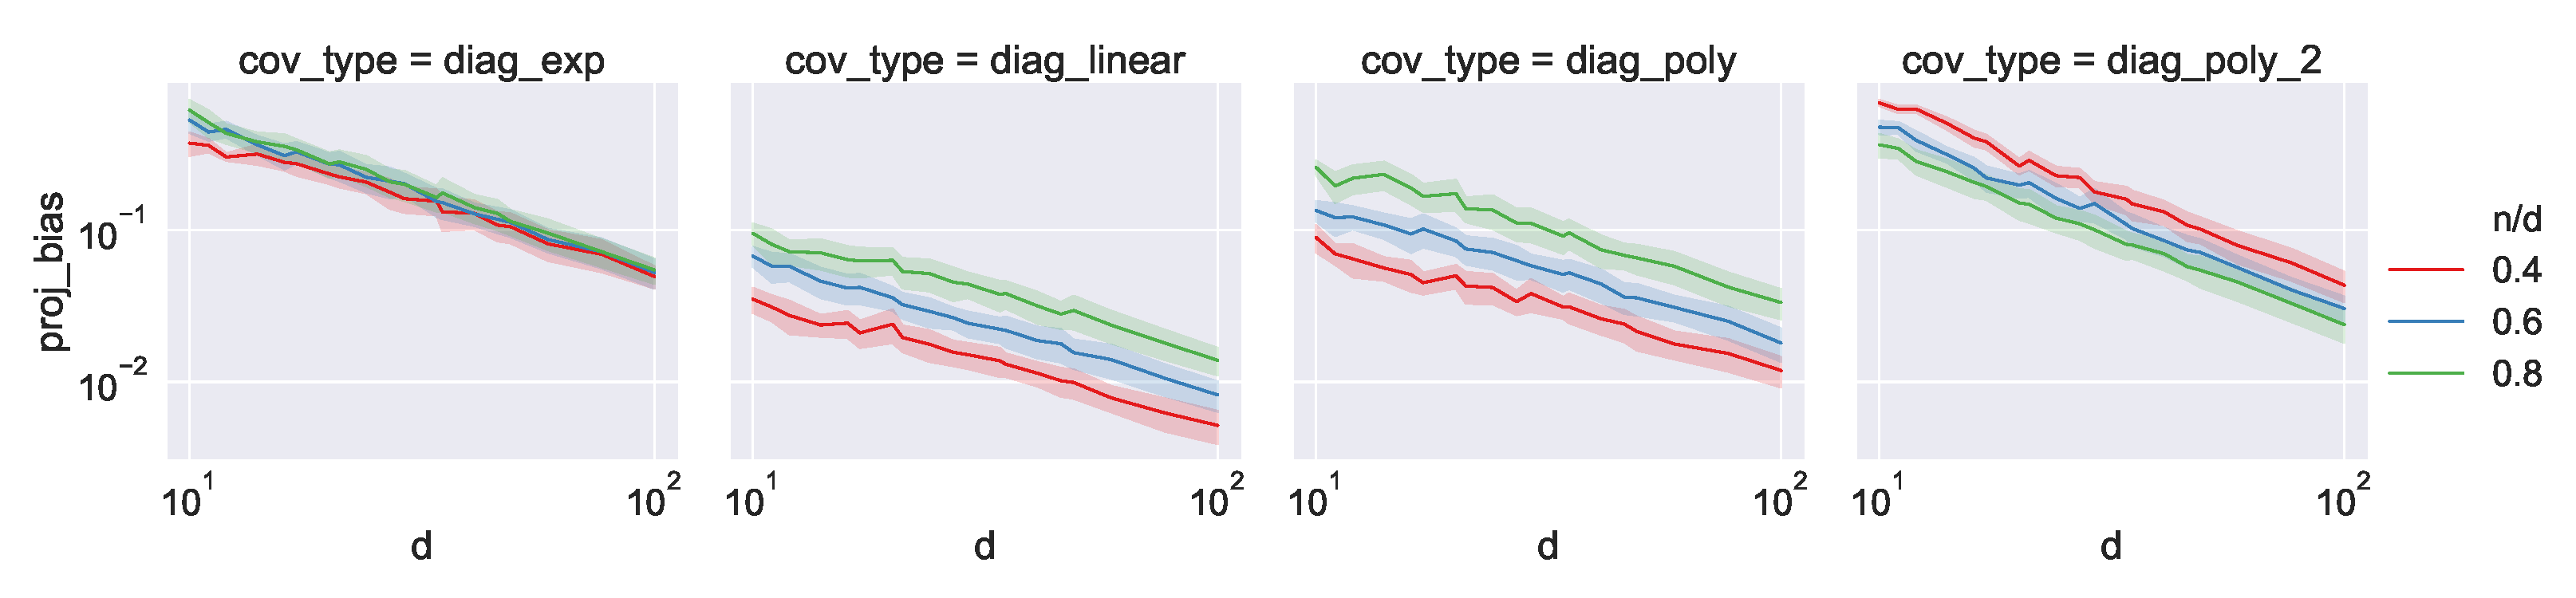
\includegraphics[width=\textwidth]{continuous_figures/proj_bias.pdf}
  \vspace{-.8cm}
  \caption{
    Empirical verification of the asymptotic consistency of surrogate MSE.
    We show the discrepancies for the variance (top) and bias
    (bottom),  with bootstrapped $95\%$ confidence intervals, as $d$
    increases and $n/d$ is fixed. We observe
     $O(1/d)$ decay (linear with slope $-1$ on a log-log plot).
  }
  \label{f:conj-wishart}
\end{figure}

Figure~\ref{f:conj-wishart} (top) plots the variance discrepancy (with
$\E[\tr((\X^\top\X)^\dagger)]$ estimated via Monte Carlo
sampling and bootstrapped confidence intervals) as $d$ increases from $10$ to
$1000$, across a range of aspect ratios $n/d$. In all cases, we observe that
the discrepancy decays to zero at a rate of $O(1/d)$.
Figure~\ref{f:conj-wishart} (bottom) plots the bias discrepancy, with the same
rate of decay observed throughout.  Note that the range of $d$ is smaller than
in Figure \ref{f:conj-wishart} (top) because the large number of Monte Carlo
samples (up to two million) required for this experiment made the computations
much more expensive (more details in Appendix \ref{a:empirical}). Based on the
above empirical results, we conclude with a conjecture.
\begin{conjecture}
  \label{c:1-over-d-rate}
  When $\mu$ is a centered multivariate Gaussian and its covariance
  has a constant condition
  number, then, for $n/d$ fixed, the surrogate MSE satisfies:
  $\big|\frac{\textnormal{MSE}[\X^\dagger\y]}{\Mc}-1\big|= O(1/d)$.
\end{conjecture}

% The results of empirically validating \Cref{c:wishart} are illustrated in
% Figure~\ref{f:conj-wishart} (top), where we performed Monte Carlo estimation of
% $\E\big[\tr((\X^\top\X)^\dagger)\big]$ and plot
% $\big|\E[\tr((\X^\top\X)^\dagger)]\,\Vc(\Sigmab,n)^{-1} -1\big|$ as $d$ increases from
% $10$ to $1000$, across a range of aspect ratios $n/d$ and eigenvalue decay
% profiles for $\Sigmab$.
% We observe that on log-log axes all of the plots are
% decreasing with a linear $-1$ slope, consistent with the $O(1/d)$ rate
% predicted by \Cref{c:wishart}. \Cref{c:projection} is handled similarly, by
% sampling $\X\sim\mu^n$ where $\mu=\Nc(\zero,\Sigmab )$ to obtain a Monte Carlo
% estimate of $\E[\I-\X^\dagger\X]$.

% Figure~\ref{f:conj-wishart} (bottom) shows how \eqref{eq:projection} decays as
% we hold the aspect ratio $n/d$ fixed and increase $d$ between $10$ and $100$
% across the listed eigenvalue decay profiles and aspect ratios. Again, we
% observe on log-log axes a linear decay with slope $-1$ consistent with the
% $O(1/d)$ rate posed by \Cref{c:projection}. Note that the range of $d$ is
% smaller than in Figure \ref{f:conj-wishart} (top) because the large number of
% Monte Carlo samples (up to two million) required for this experiment made the
% computations much more expensive.


